\documentclass[letterpaper, twoside, 12pt,memoire]{thETS}
\interdisplaylinepenalty=2500
\usepackage{amsmath}
\usepackage{amsfonts}
\usepackage{amssymb}
\usepackage[utf8]{inputenc}
\usepackage{graphicx}
\usepackage{color}
\usepackage[T1]{fontenc}
\usepackage{subfigure}
\usepackage{setspace}
\usepackage{todonotes}
\usepackage{varwidth}
\usepackage[round]{natbibETS}
%\usepackage{url}

\newcommand{\LT}[1]{%
	{
	\todo[inline,color={red!33!green!33!blue!33}]{%
	\textbf{[LT]:}~#1}
	}}
	
\newcommand{\SC}[1]{%
	{
	\todo[inline,color={red!100!green!33}]{%
	\textbf{[SC]:}~#1}
	}}

\newcommand{\ltCodec}{logiciel de référence H.264/AVC JM}
\newcommand{\fig}[1]{figure~\ref{#1}}
\newcommand{\ang}[1]{(\textit{#1})}
%DIF PREAMBLE EXTENSION ADDED BY LATEXDIFF
%DIF UNDERLINE PREAMBLE %DIF PREAMBLE
\RequirePackage[normalem]{ulem} %DIF PREAMBLE
\RequirePackage{color}\definecolor{RED}{rgb}{1,0,0}\definecolor{BLUE}{rgb}{0,0,1} %DIF PREAMBLE
\providecommand{\DIFadd}[1]{{\protect\color{blue}\uwave{#1}}} %DIF PREAMBLE
\providecommand{\DIFdel}[1]{{\protect\color{red}\sout{#1}}}                      %DIF PREAMBLE
%DIF SAFE PREAMBLE %DIF PREAMBLE
\providecommand{\DIFaddbegin}{} %DIF PREAMBLE
\providecommand{\DIFaddend}{} %DIF PREAMBLE
\providecommand{\DIFdelbegin}{} %DIF PREAMBLE
\providecommand{\DIFdelend}{} %DIF PREAMBLE
%DIF FLOATSAFE PREAMBLE %DIF PREAMBLE
\providecommand{\DIFaddFL}[1]{\DIFadd{#1}} %DIF PREAMBLE
\providecommand{\DIFdelFL}[1]{\DIFdel{#1}} %DIF PREAMBLE
\providecommand{\DIFaddbeginFL}{} %DIF PREAMBLE
\providecommand{\DIFaddendFL}{} %DIF PREAMBLE
\providecommand{\DIFdelbeginFL}{} %DIF PREAMBLE
\providecommand{\DIFdelendFL}{} %DIF PREAMBLE
%DIF END PREAMBLE EXTENSION ADDED BY LATEXDIFF

\begin{document}
\begin{chapter}{Résultats et analyse}
\DIFdelbegin \DIFdel{Les }\DIFdelend \DIFaddbegin \DIFadd{Au chapitre précédent, nous avons présenté les concepts théoriques des nouvelles }\DIFaddend approches sélectives \DIFaddbegin \DIFadd{proposées, }\DIFaddend basées sur le MCB et le SDMCB \DIFdelbegin \DIFdel{ont été démontrées
théoriquement au chapitre précédent. Maintenant, nous effectuons }\DIFdelend \DIFaddbegin \SC{On utilise des acronymes français ou anglais pour cela? }\DIFadd{. Dans ce chapitre, nous faisons état }\DIFaddend des essais pratiques \DIFdelbegin \DIFdel{afin d'attester des }\DIFdelend \DIFaddbegin \DIFadd{réalisés pour valider les }\DIFaddend gains réalisables \DIFaddbegin \DIFadd{à l'aide de ces approches }\DIFaddend dans des conditions \DIFdelbegin \DIFdel{similaires
à celles rencontrées par des applications }\DIFdelend de vidéo mobile. 
\DIFdelbegin \DIFdel{Dans ce chapitre,
nous }\DIFdelend \DIFaddbegin \DIFadd{Nous }\DIFaddend démontrons, non seulement l'efficacité des approches sélectives \DIFaddbegin \DIFadd{proposées}\DIFaddend , mais
aussi \DIFdelbegin \DIFdel{sa }\DIFdelend \DIFaddbegin \DIFadd{leur }\DIFaddend supériorité par rapport à l'approche de dissimulation utilisée par le
décodeur inclus avec le \ltCodec.



%DIFDELCMD < %%%
\DIFdel{À la }%DIFDELCMD < \fig{fig-726}%%%
\DIFdel{, nous présentons}\DIFdelend \DIFaddbegin \DIFadd{Nous débutons par présenter nos hypothèses de validation à la section \ref{sec-Hypotheses-validation}.
Nous expliquons ensuite}\DIFaddend , à \DIFdelbegin \DIFdel{titre d'exemple, des trames issues de la $726^{\text{e}}$ sous-séquence de notre jeu de tests. Les }\DIFdelend \DIFaddbegin \DIFadd{la section \ref{sec-bancEssai}, les }\DIFaddend composantes de notre
banc d'essai \DIFdelbegin \DIFdel{, utilisé }\DIFdelend \DIFaddbegin \DIFadd{utilisées }\DIFaddend pour créer \DIFdelbegin \DIFdel{ce }\DIFdelend \DIFaddbegin \DIFadd{notre }\DIFaddend jeu de tests\DIFdelbegin \DIFdel{, sont expliquées à la section
\ref{sec-bancEssai}. L'image erronée }%DIFDELCMD < \subref{fig-726-bad} %%%
\DIFdel{permet la
visualisation du résultat obtenu par le }\DIFdelend \DIFaddbegin \DIFadd{. Dans le but de valider nos hypothèse sur le décodeur, les
taux de succès observés lors du }\DIFaddend décodage d'une \DIFdelbegin \DIFdel{tranche corrompue. Les
probabilités de réussir un tel décodage }\DIFdelend \DIFaddbegin \DIFadd{séquence erronnée }\DIFaddend sont présentées à la section
\ref{sec-ResilienceDecodeur} \DIFdelbegin \DIFdel{. Tandis qu'}\DIFdelend \DIFaddbegin \SC{je ne parle pas de probabilité car c'est un événement mesuré, pas théorique}\DIFadd{. Un succès sera considéré lorsque le décodeur retournera une image sans planter}\SC{trouver mieux que planter}\DIFadd{. Finalement, }\DIFaddend à la section
\ref{sec-ApprocheSelective}, nous \DIFdelbegin \DIFdel{mesurons }\DIFdelend \DIFaddbegin \DIFadd{présentons }\DIFaddend les résultats obtenus de
l'application de nos algorithmes de détection et dissimulation d'erreurs sur
\DIFdelbegin \DIFdel{cette image }\DIFdelend \DIFaddbegin \DIFadd{les images décodées}\DIFaddend .
\DIFaddbegin 


\begin{section}{Hypothèses de validation}
\label{sec-Hypotheses-validation}

\DIFadd{Débutons par énumérer les hypothèses faites dans le cadre de nos expérimentations. 
À la }\fig{fig-726}\DIFadd{, nous présentons, à titre d'exemple, des trames issues de la
$726^{\text{e}}$ sous-séquence de notre jeu de tests (expliqué plus en détail à la section suivante).  L'image erronée }\subref{fig-726-bad} \DIFadd{correspond au résultat obtenu par le décodage d'une tranche corrompue. 
}


\begin{figure}[htb]
\DIFaddFL{\fbox{\begin{varwidth}{\textwidth}\centering
\subfigure[Trame précédente]{
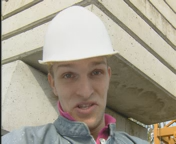
\includegraphics[width=0.46\linewidth]{images/prevForeman.png}
\label{fig-726-prev}
}
\subfigure[Trame erronée]{
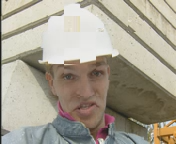
\includegraphics[width=0.46\linewidth]{images/badForeman.png}
\label{fig-726-bad}
}
\subfigure[Dissimulation par tranche calquée]{
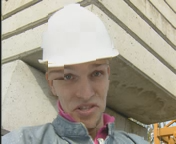
\includegraphics[width=0.46\linewidth]{images/fcForeman.png}
\label{fig-726-sc}
}
\subfigure[Trame de référence]{
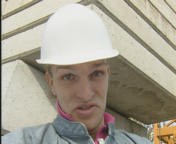
\includegraphics[width=0.46\linewidth]{images/perfForeman.png}
\label{fig-726-perf}
}
\end{varwidth}}
}\caption{\DIFaddFL{Les trames résultantes de la sous-séquence }\#\DIFaddFL{726 du jeu de tests
(Séquence~: Foreman, QP=16 BER=0.0008, FMO=Dispersé)}}
\label{fig-726}
\end{figure}
\SC{pour la figure 1, il me semble que tu ne peux pas mettre les descriptions dans les figures et il fait les mettre dans la description globale de la figure}

\DIFaddend La trame qui précède l'erreur \subref{fig-726-prev} ne contient
jamais d'erreurs, une \DIFdelbegin \DIFdel{supposition }\DIFdelend \DIFaddbegin \DIFadd{hypothèse }\DIFaddend posée aussi par~\citep{Superiori2007}. Nous
\DIFdelbegin \DIFdel{avons }\DIFdelend \DIFaddbegin \DIFadd{aurons }\DIFaddend recours à cette trame comme source de contenu pour la dissimulation
d'erreurs de la trame \subref{fig-726-bad}. La trame \subref{fig-726-sc} est
celle reconstruite à l'aide du calquage de la tranche de la trame précédente
\subref{fig-726-prev}. Cette trame représente la solution d'un décodeur moderne,
ce à quoi nous allons comparer nos dissimulations. La figure
\subref{fig-726-perf} est la trame de référence, qui n'a pas subit l'encodage.
C'est la trame que nous utilisons pour mesurer le PSNR.
\DIFaddbegin \SC{mettre toutes tes hypothèses ici}\DIFadd{. 
}\end{section}
\DIFaddend 

\begin{section}{Description du banc d'essai}
\label{sec-bancEssai}
Afin \DIFdelbegin \DIFdel{d'étudier nos hypothèses sur la détection de la vraisemblance de régions
d'images}\DIFdelend \DIFaddbegin \DIFadd{de valider notre notre approche de détection et de dissimulation vidéo}\DIFaddend , nous avons construit un banc d'essai constitué d'un grand nombre de\DIFaddbegin \SC{il me semble que la phrase d'avant n'avait pas de sens. il me semble que tu n'étudie pas tes hypothèses, enfin ce n'est pas le but premier du banc d'essaie. De plus du n'étudie pas tes hypothèses sur la détection de la vraisemblance de régions d’images. C'est quoi une détection de la vraisemblance? On fait une détection ou on évalue la vraisemblance mais il me semble qu'on ne fait pas une détection de la vraisemblance}
\DIFaddend séquences vidéos \DIFaddbegin \DIFadd{encodées à divers débits et }\DIFaddend soumises à des taux d'erreurs \DIFdelbegin \DIFdel{, }\DIFdelend similaires à ceux proposés dans
l'ouvrage \citep{Stockhammer2003}. Ces \DIFdelbegin \DIFdel{taux représentent les conditions
présentes lors du }\DIFdelend \DIFaddbegin \DIFadd{erreurs découlent des conditions
difficiles de }\DIFaddend transport de séquences vidéo H.264 vers des appareils \DIFaddbegin \DIFadd{évoluant sur des réseau }\DIFaddend mobiles.

\begin{figure}[htb]
\fbox{
\centering
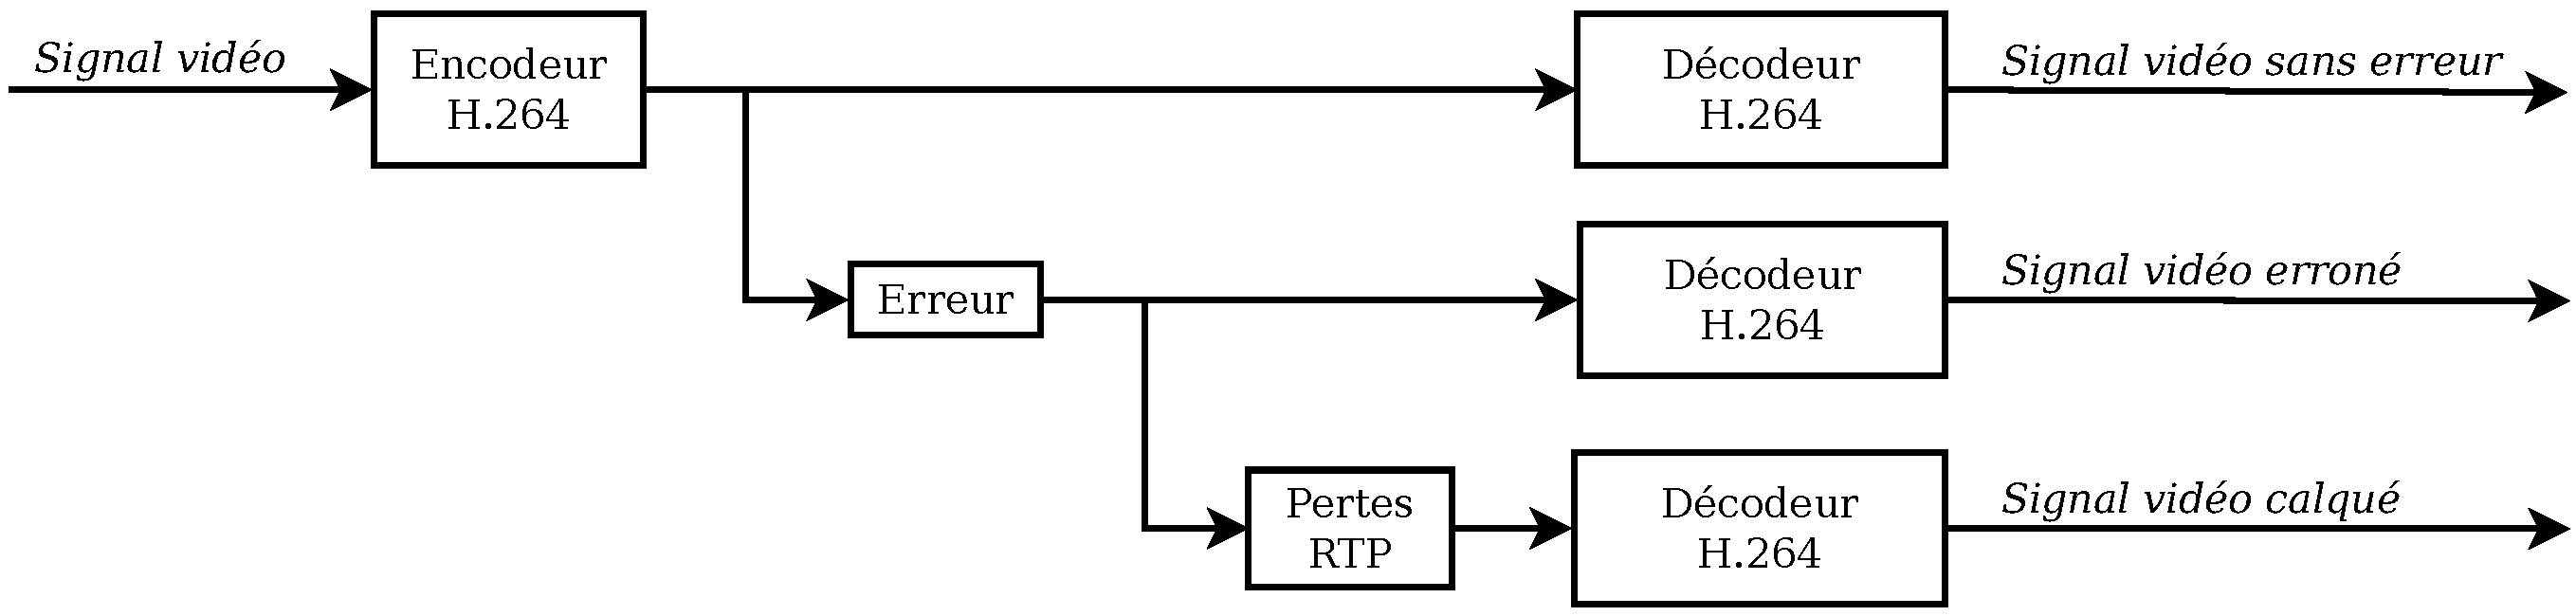
\includegraphics[width=0.97\linewidth]{images/EncoderDecoder.pdf}
}
\caption{Diagramme des étapes du banc d'essai}
\label{fig-EncoderDecoder}
\end{figure}
\DIFaddbegin \SC{les boites des 3 décodeurs devrait être toutes pareilles et chacune devrait avoir une sortie avec un nom différent: signal vidéo sans erreur, signal vidéo erroné, signal vidéo calqué ou quelque chose du genre}
\DIFaddend 

Nous présentons, à la \fig{fig-EncoderDecoder}, les étapes de notre banc
d'essai. \DIFdelbegin \DIFdel{En résumé, }\DIFdelend \DIFaddbegin \DIFadd{Nous y observons qu'}\DIFaddend un signal vidéo est encodé\DIFaddbegin \DIFadd{, transmis, }\DIFaddend puis décodé trois fois.  La
première opération de décodage décode les données sans que celles-ci soient
exposées à l’erreur. Cette étape est cruciale afin de déterminer la dégradation
visuelle engendrée par l’encodage du signal \DIFdelbegin \DIFdel{. Par la suite}\DIFdelend \DIFaddbegin \SC{on mesure vraiment l'effet de l'encodage ou bien ça sert plutôt de référence pour mesurer les erreurs de transport}\DIFadd{. Dans la seconde opération}\DIFaddend , la séquence encodée
est sujette à un motif d’erreur binaire \ang{Bit Error Pattern} gaussien. Les
données corrompues sont envoyées au décodeur\DIFdelbegin \DIFdel{, s}\DIFdelend \DIFaddbegin \DIFadd{. S}\DIFaddend ’il réussit à les décoder,
celles-ci sont conservées, sinon la sous-séquence est rejetée. En dernier lieu,
la sous-séquence corrompue est analysée par un module de détection de pertes RTP
\ang{RTP loss}. Celui-ci identifie et retire les paquets RTP corrompus. Les
données résultantes de l’analyse de pertes RTP sont décodées. Lorsque le
décodeur \DIFaddbegin \DIFadd{s'}\DIFaddend aperçoit \DIFaddbegin \DIFadd{d'}\DIFaddend un paquet manquant, il \DIFdelbegin \DIFdel{procède à utiliser }\DIFdelend \DIFaddbegin \DIFadd{utilise }\DIFaddend une approche de
dissimulation d’erreurs,  \DIFdelbegin \DIFdel{soit }\DIFdelend en remplaçant\DIFaddbegin \DIFadd{, par exemple, }\DIFaddend la tranche manquante par son
équivalent dans la trame précédente\footnoteETS{Dans cet ouvrage, \textit{slice
copy} a été utilisé au détriment de \textit{motion copy}, car aucune
implémentation fonctionnelle de \textit{motion copy} était disponible. Nous
avons eux des problèmes lors de l'utilisation de \textit{motion copy} avec les
versions~15.1 à 16.2 du décodeur inclus dans le \ltCodec. Ces problèmes sont
connus et confirmés par plusieurs forums internet et catalogués dans le
logiciel de suivi de problèmes Mantis relié au \ltCodec~\citep{BUG}. Quoique
notre ouvrage est aussi compatible avec \textit{motion copy}, c'est pour
cette raison, que nous avons testé uniquement avec \textit{slice copy}.}
(\textit{slice copy}, traduit dans cet ouvrage par la locution tranche calquée).\DIFaddbegin \SC{revoir cette phrase}
\DIFaddend 

Les séquences sont encodées et décodées à l'aide de la
version~16.2 du \ltCodec~\citep{JM}. Ce dernier, n'étant pas un produit
commercial, a pour objectif principal la démonstration de nouvelles
fonctionnalités visant la norme H.264. Notre banc d'essai est constitué de
sous-ensembles de quatre trames consécutives commençant à un emplacement
aléatoire \DIFaddbegin \DIFadd{dans diverses séquences vidéos}\DIFaddend . Ces sous-ensembles débutent par une trame \textit{intra} et trois
trames \textit{inter} (IPPP). Nous retenons cinq sous-ensembles pour chaque
séquence de résolution QCIF contenue dans l'ensemble de séquences de référence
de \DIFaddbegin \DIFadd{l'Université de l'Arizona}\DIFaddend ~\citep{YUV}.
\LT{Définir QCIF dans la section transport de vidéo.}

Dans le contexte d'applications mobiles, le débit est souvent fixe (\DIFaddbegin \DIFadd{typiquement entre }\DIFaddend 64~kb/s \DIFdelbegin \DIFdel{,
}\DIFdelend \DIFaddbegin \DIFadd{et
}\DIFaddend 128~kb/s \DIFdelbegin \DIFdel{\ldots}\DIFdelend \DIFaddbegin \DIFadd{pour les séquences QCIF}\DIFaddend ). Cependant, pour simplifier nos expérimentations, nous
imposons \DIFaddbegin \DIFadd{plutôt }\DIFaddend un pas de quantification (QP) fixe. Ceci élimine les variations de \DIFdelbegin \DIFdel{PSNR
dû }\DIFdelend \DIFaddbegin \DIFadd{qualité, mesurées à l'aide du PSNR}\LT{Définir PSNR}\DIFadd{,
dus }\DIFaddend aux changements de QP requis pour garder le débit fixe. Les indices de pas de
quantifications \DIFaddbegin \DIFadd{utilisés }\DIFaddend sont~: 16, 20, 24 et 28. Ces valeurs sont choisies, car elles
représentent un intervalle de données plausibles pour une application mobile
selon la bande passante disponible. De plus, nous n'avons pas retenu des QP trop
élevés (>30), car la quantité de bits requis pour encoder une trame est
tellement faible qu’il arrive souvent, que les taux d’erreurs utilisés ne
parviennent pas à briser un seul bit de la trame. \DIFaddbegin \SC{mettre une petite note que les QP varient entre 0 et 51}
\DIFaddend 

Les taux d'erreur binaire (BER) utilisés sont~: 0.0004, 0.0008, 0.0016, et
0.0032. Cet intervalle de taux est considérablement large et agressif par rapport aux
intervalles d'erreurs retrouvés dans la littérature de la norme
H.264~\citep{Stockhammer2003}. Nous avons \DIFdelbegin \DIFdel{pris }\DIFdelend \DIFaddbegin \DIFadd{choisi }\DIFaddend un tel
intervalle pour obtenir des résultats témoignant des gains possibles dans un
grand nombre de conditions d'erreur de transport. Le taux d'erreur utilisé est
appliqué au niveau des bits et non pas au niveau des paquets~\citep{Wenger2003}
ou des blocs (comme dans les ouvrages de dissimulation d'erreurs). 

Seulement la troisième trame (une trame P) est exposée à l'erreur. En ce qui
concerne l'ordonnancement de macroblocs flexible (FMO), deux types sont
employés~: dispersé \ang{dispersed} et entrelacé \ang{interlaced}. Tous deux
sont composés de deux tranches. À la \fig{fig-392} et \DIFdelbegin \DIFdel{\ref{fig-726}}\DIFdelend \DIFaddbegin \DIFadd{\ref{fig-1752}}\DIFaddend , nous présentons
deux exemples d'erreurs pour chacun des types d'ordonnancement. Les
sous-séquences sont encodées à 30 images par seconde, tandis que les autres
paramètres sont propres au profil de base \ang{baseline} défini dans la norme
H.264. Le format de sortie est RTP et la résolution est QCIF, c'est-à-dire
$176\times 144$ pixels. Cependant, les en-têtes NAL et RTP n'ont pas été exposés
à l'erreur.

\begin{figure}[htb]
\fbox{\begin{varwidth}{\textwidth}\centering
\subfigure[Trame erronée]{

\includegraphics[width=0.46\linewidth]{images/badCarphoneInterleaved.png}
\label{fig-392-bad}
}
\subfigure[Erreur (amplifiée)]{
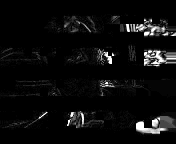
\includegraphics[width=0.46\linewidth]{images/diffCarphoneInterleaved.png}
\label{fig-392-err}
}
\end{varwidth}}
\caption{Exemple de l'erreur présente dans la sous-séquence \#392 du jeu de
tests (Séquence~: Carphone, QP=16 BER=0.0032, FMO=Dispersé)}
\label{fig-392}
\end{figure}

\begin{figure}[htb]
\fbox{\begin{varwidth}{\textwidth}\centering
\subfigure[Trame erronée]{
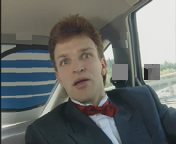
\includegraphics[width=0.46\linewidth]{images/badCarphoneDispersed.png}
\label{fig-1752-bad}
}
\subfigure[Erreur (amplifiée)]{
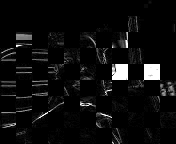
\includegraphics[width=0.46\linewidth]{images/diffCarphoneDispersed.png}
\label{fig-1752-err}
}
\end{varwidth}}
\caption{Exemple de l'erreur présente dans la sous-séquence
\#1752 du jeu de tests (Séquence~: Carphone, QP=16 BER=0.0032, FMO=Entrelacé)}
\label{fig-1752}
\end{figure}
\DIFaddbegin \SC{Il me semble que les figures sont inversées. La première est interleaved (entrelacé) et la seconde dispersed}
\DIFaddend 

Notre banc d'essai est constitué d'un jeu de tests de 2720 sous-ensembles de
trames, Plus précisément, \DIFaddbegin \DIFadd{nous avons }\DIFaddend 1360 trames dispersées et 1360 trames entrelacées.
Dans la prochaine section, \DIFdelbegin \DIFdel{il sert }\DIFdelend \DIFaddbegin \DIFadd{ce banc d'essai servira }\DIFaddend à déterminer la résilience du décodeur inclus
dans le \ltCodec. À la section~\ref{sec-ApprocheSelective}, il \DIFdelbegin \DIFdel{est }\DIFdelend \DIFaddbegin \DIFadd{sera }\DIFaddend utilisé pour
valider nos approches sélectives de détection et de dissimulation d'erreur.
\DIFaddbegin 

\SC{Tu dois expliquer comment tu arrives à 1360. 1360 = N séquences x 4 taux erreur x 4 QP x etc.}
\SC{!!!!! Très important!!!! Ta méthodologie quant aux séquences utiliées pour entraîner ton algorithme (e.x. trouver le bon seuil) versus établir les performances sera scrutée à la loupe. Tu ne peux pas entraîner sur le même contenu sur lequel tu mesure les performances. Tu dois présenter sur quoi tu entraînes et sur quoi tu évalues la performance.}

\DIFaddend \end{section}

\DIFdelbegin %DIFDELCMD < \begin{section}{Analyse de la résilience du décodeur}
%DIFDELCMD < %%%
\DIFdelend \DIFaddbegin \begin{section}{Analyse de la résilience aur erreurs du décodeur de référence H.264}
\DIFaddend \label{sec-ResilienceDecodeur}
Dans certaines conditions, le décodeur fournit avec le \ltCodec~réussi à décoder
des séquences binaires corrompues. Cette découverte, initiatrice de notre effort
de recherche, fut réalisée très tôt dans nos expérimentations.  Nous définissons
un décodage réussi comme~: l'opération de décoder une tranche corrompue sans
causer de défaillances \ang{crash} chez le décodeur, sans pour autant garantir
l'intégrité \DIFdelbegin \DIFdel{de }\DIFdelend \DIFaddbegin \DIFadd{du }\DIFaddend contenu résultant. En d'autres mots, l'image issue du décodage
d'une tranche corrompue va souvent contenir de la dégradation visuelle (voir
figures \ref{fig-726-bad}, \ref{fig-392-bad} et \ref{fig-1752-bad}). Le taux de
décodages réussis varie, non seulement selon le taux d'erreur binaire appliqué à la séquence, mais aussi à l'égard du paramètre
de quantification (QP) utilisé lors de l'encodage. Ceci s'explique par le fait
qu'un QP plus faible \DIFdelbegin \DIFdel{requiert }\DIFdelend \DIFaddbegin \DIFadd{force l'encodeur à utiliser }\DIFaddend plus de bits pour encoder une trame\DIFdelbegin \DIFdel{, }\DIFdelend \DIFaddbegin \DIFadd{; et }\DIFaddend plus il y a
de bits sujets à \DIFdelbegin \DIFdel{l'erreur , }\DIFdelend \DIFaddbegin \DIFadd{erreur et }\DIFaddend plus la probabilité de corruption de la trame
augmente.

\begin{figure}[htb]
\fbox{\begin{varwidth}{\textwidth}\centering
\subfigure[Ordonnacement dispersé]{
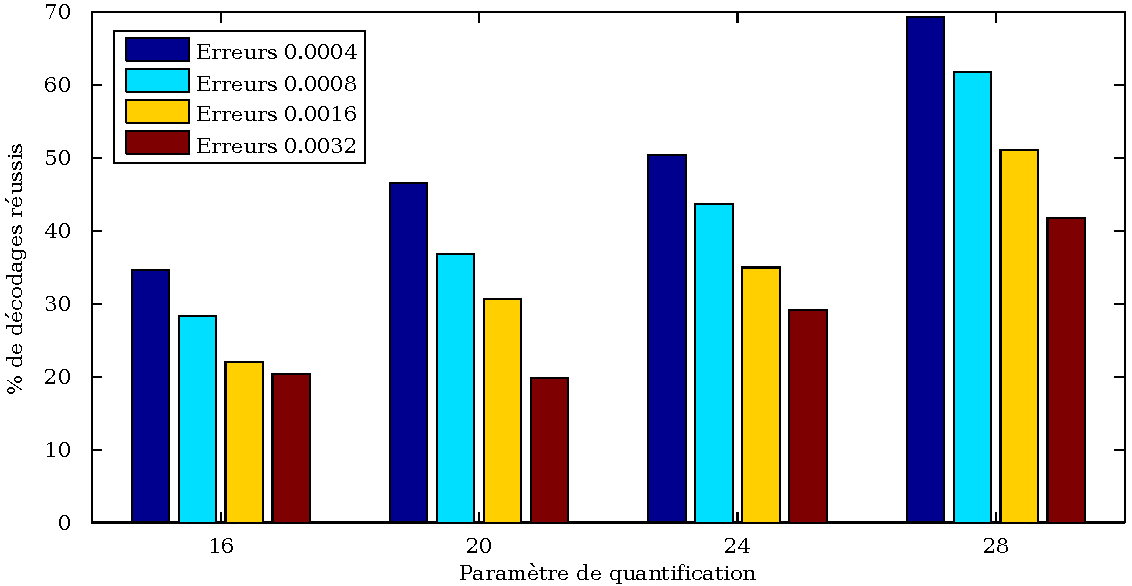
\includegraphics[width=0.97\linewidth]{images/decodingDispersed.pdf}
}\\
\subfigure[Ordonnacement entrelacé]{
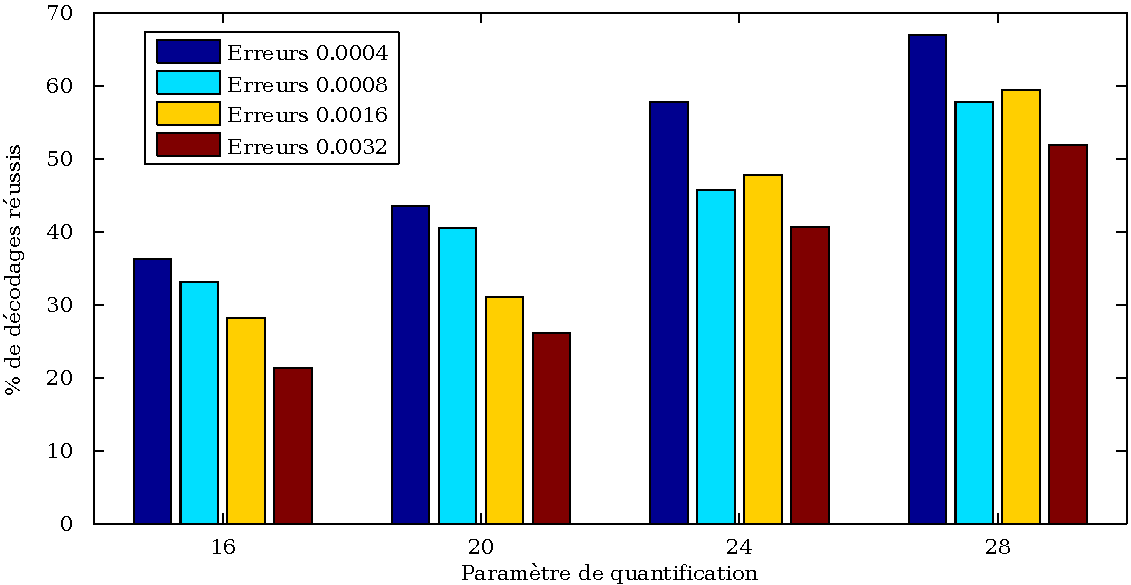
\includegraphics[width=0.97\linewidth]{images/decodingInterleaved.pdf}
}
\end{varwidth}}
\caption{Histogrammes des pourcentages de décodages réussis en fonction du
paramètre de quantification utilisé lors de l'encodage ainsi que du taux
d'erreurs \DIFdelbeginFL \DIFdelFL{binaires }\DIFdelendFL \DIFaddbeginFL \DIFaddFL{sur les bits }\DIFaddendFL (BER). }
\label{fig-Decodings}
\end{figure}
\DIFaddbegin \SC{Ajuster les axes des y car je ne crois pas que les taux de réussites soient de 0.3 pourcent }
\DIFaddend 

\DIFdelbegin \DIFdel{L'histogramme }\DIFdelend \DIFaddbegin \DIFadd{Les histogrammes }\DIFaddend de la \fig{fig-Decodings} \DIFdelbegin \DIFdel{décrit }\DIFdelend \DIFaddbegin \DIFadd{présentent }\DIFaddend les taux de décodages
réussis observés en fonction des paramètres de quantification et \DIFaddbegin \DIFadd{du }\DIFaddend taux d'erreurs
\DIFdelbegin \DIFdel{binaires }\DIFdelend \DIFaddbegin \DIFadd{sur les bits }\DIFaddend présents dans notre jeu de tests. Ces taux sont intéressants, car ils
confirment que le décodage des données corrompues peut avoir un taux de réussite
allant de 20~\% à 70~\%, selon les conditions. On peut concevoir une stratégie
de résilience à l'erreur, où une prochaine génération de décodeurs \DIFdelbegin \DIFdel{serait }\DIFdelend \DIFaddbegin \DIFadd{seraient }\DIFaddend en
mesure d'effectuer une tentative de décodage d'une tranche corrompue, dans un
environnement contrôlé (possiblement un second décodeur), afin de contrer
l'impact d'une défaillance.\DIFaddbegin \SC{Pas clair, clarifier l'idée. c'est quoi contrer l'impact de la défaillance }
\DIFaddend 

\begin{figure}[htb]
\fbox{\begin{varwidth}{\textwidth}\centering
\subfigure[Trame Corrompue]{
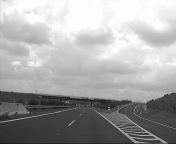
\includegraphics[width=0.30\linewidth]{images/ErrorFrame.png}
\label{fig-ErrorFrame}
}
\subfigure[Différentiel de \subref{fig-ErrorFrame} et la trame non-erronée]{
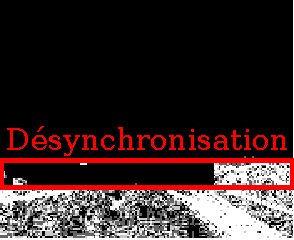
\includegraphics[width=0.30\linewidth]{images/Desync.pdf}
\label{fig-Desync}
}
\subfigure[Différentiel de \subref{fig-ErrorFrame} et la trame précédente]{
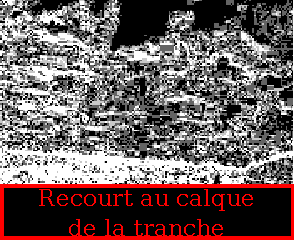
\includegraphics[width=0.30\linewidth]{images/Revert.pdf}
\label{fig-Revert}
}
\end{varwidth}}
\caption{Exemple du comportement du décodeur. En \subref{fig-Desync}, le
différentiel de \subref{fig-ErrorFrame}, par rapport à la trame
\DIFdelbeginFL \DIFdelFL{encodée, mais non erroné}\DIFdelendFL \DIFaddbeginFL \DIFaddFL{codée/décodée sans erreur}\DIFaddendFL , est utilisé pour démontrer la désynchronisation. Le
différentiel entre \subref{fig-ErrorFrame} et la trame précédente permet de démontrer, en
\subref{fig-Revert}, l'utilisation du calque de tranche.}
\label{fig-DecoderBehavior}
\end{figure}

Lors du décodage d'une tranche corrompue, le décodeur inclus dans le
\ltCodec~fait la transition entre trois états distincts. Le résultat de ceux-ci
est illustré à la \fig{fig-DecoderBehavior}. Le premier état est celui du
décodage des bits de la tranche corrompue situés avant l'erreur. Cet état est
équivalant au décodage normal d'une trame. Il est illustré par la partie
supérieure, tout en noir (signifiant l'absence de différence), du
différentiel~\subref{fig-Desync} de la \fig{fig-DecoderBehavior}.

Par la suite, le décodeur décode le premier bit corrompu. Ceci cause une
désynchronisation des codes binaires de l'encodage entropique. Même si les
autres bits de la séquence sont valides, la désynchronisation fait en sorte
qu'ils sont associés à la mauvaise valeur dans la table de référence CAVLC. Le
décodeur interprète ces mauvaises valeurs\DIFdelbegin \DIFdel{ce qui entraine }\DIFdelend \DIFaddbegin \DIFadd{; ce qui entraîne }\DIFaddend une dégradation
visuelle dans l'image. Cette dégradation peut se manifester fortement comme
c'est le cas dans l'image de la \fig{fig-726-bad} ou être presque imperceptible,
comme \DIFdelbegin \DIFdel{celle }\DIFdelend \DIFaddbegin \DIFadd{c'est le cas }\DIFaddend dans la \fig{fig-ErrorFrame}. Afin de mieux voir la dégradation
visuelle de la \fig{fig-ErrorFrame}, elle est encadrée à la \fig{fig-Desync}.
C'est dans ce second état que le décodeur est le plus vulnérable aux
défaillances.

Le second état se termine lorsque le décodeur cesse d'insérer de la dégradation
visuelle dans l'image et utilise le contenu provenant de la tranche précédente.
Ce changement est illustré en~\ref{fig-Revert}. Ici, on suppose que le décodeur
est complètement désynchronisé, il ne sait que faire de ce qu'il décode, il
applique donc le contenu des blocs précédents, ce qui, grâce à la corrélation
temporelle, est le contenu de remplacement correct, s'il y a absence de
mouvement. De plus, notons \DIFaddbegin \DIFadd{que }\DIFaddend dans l'image~\ref{fig-ErrorFrame}, il y a très peu
d'effet de blocs causés par la désynchronisation. Ceci est dû au filtre
antiblocs\DIFdelbegin \DIFdel{, lorsqu}\DIFdelend \DIFaddbegin \DIFadd{. Lorsqu}\DIFaddend 'il est appliqué sur la trame, il va identifier et lisser les
effets de blocs. Ceci explique aussi pourquoi, à la \fig{fig-392-bad}, l'erreur
se répand à la tranche non erronée. Dans ce cas, le filtre antiblocs lisse le
bloc erroné, ce qui répand l'erreur dans les blocs avoisinants.
\DIFaddbegin 

\SC{Je ne suis pas trop certain de l'explication que le décodeur applique les blocs précédents. Est-ce vraiment ce qui se passe? C'est pas que le décodeur a un buffeur d'image décodé et qu'il l'écrase lors du décodage d'une nouvelle trame. S'il abandonne avant de terminer le décodage d'une trame, il reste du contenu résuduel appartenant à la trame précédente. }
\DIFaddend \end{section}

\begin{section}{Analyse de l'approche sélective}
\label{sec-ApprocheSelective}
Comme démontré dans la section précédente, l'image résultante \DIFdelbegin \DIFdel{de la }\DIFdelend \DIFaddbegin \DIFadd{d'une }\DIFaddend tranche
corrompue peut \DIFaddbegin \DIFadd{souvent }\DIFaddend être décodée\DIFdelbegin \DIFdel{, ce qui la rend disponible pour guider un
algorithme de dissimulation d'erreur}\DIFdelend . Cependant, celle-ci possède, dû à la
désynchronisation du décodeur lors du décodage, une \DIFdelbegin \DIFdel{certaine }\DIFdelend dégradation
visuelle \DIFdelbegin \DIFdel{. Un }\DIFdelend \DIFaddbegin \DIFadd{plus ou moins importante. Elle peut toutefois être utilisée pour guider un
algorithme de dissimulation d'erreur grâce à un }\DIFaddend nouveau type d'algorithme \DIFdelbegin \DIFdel{, celui }\DIFdelend permettant la détection de
\DIFaddbegin \DIFadd{la }\DIFaddend dégradation visuelle \DIFdelbegin \DIFdel{est requis}\DIFdelend \DIFaddbegin \DIFadd{proposé dans ce mémoire}\DIFaddend .

L'algorithme de détection basé la mesure des effets de blocs compensés par le
mouvement (MCB), présenté dans cet ouvrage, permet la détection d'un type de
dégradation visuelle, celui causant des effets de blocs absents de la trame
précédente. La prémisse de notre approche sélective est de déterminer 
entre le calque de la tranche (\fig{fig-726-sc}) et la tranche corrompue
(\fig{fig-726-bad}), celui qui produirait la meilleure dissimulation (\DIFdelbegin \DIFdel{maximize
PSNR }\DIFdelend \DIFaddbegin \DIFadd{c.-à-d. produisant le meilleur PSNR par rapport à la trame de référence}\SC{trame décodée sans erreur ou la trame originale?}\DIFaddend ). Cette opération peut être accomplie à deux niveaux~: celui de la tranche,
à l'aide du SDMCB, ou des blocs, avec le MCB. Nous allons tout d'abord présenter
la configuration de notre banc de tests pour mesurer l'approche sélective. Par
la suite, la sous-section~\ref{sec-AnalyseSDMCB} présente les résultats
obtenus avec le SDMCB et les résultats du MCB sont présentés à la
sous-section~\ref{sec-AnalyseMCB}.
\LT{MCB, SDMCB et le PSNR sont présentés dans des séctions précédentes.}
\DIFaddbegin \SC{Les termes bancs d'essai utilisé à la section 1.1 et bancs de tests utilisés ici sont mélangeant pour le lecteur. Il faut clarifier chacun. Par exemple données d'essai devrait être utilisé à la section 1.1 dans le titre et banc d'essai pour la section actuelle. Le banc d'essai utilise les données d'essai. Le terme banc de tests n'existe pas dans le grand Dic }
\DIFaddend 

\begin{figure}[htb]
\fbox{\centering
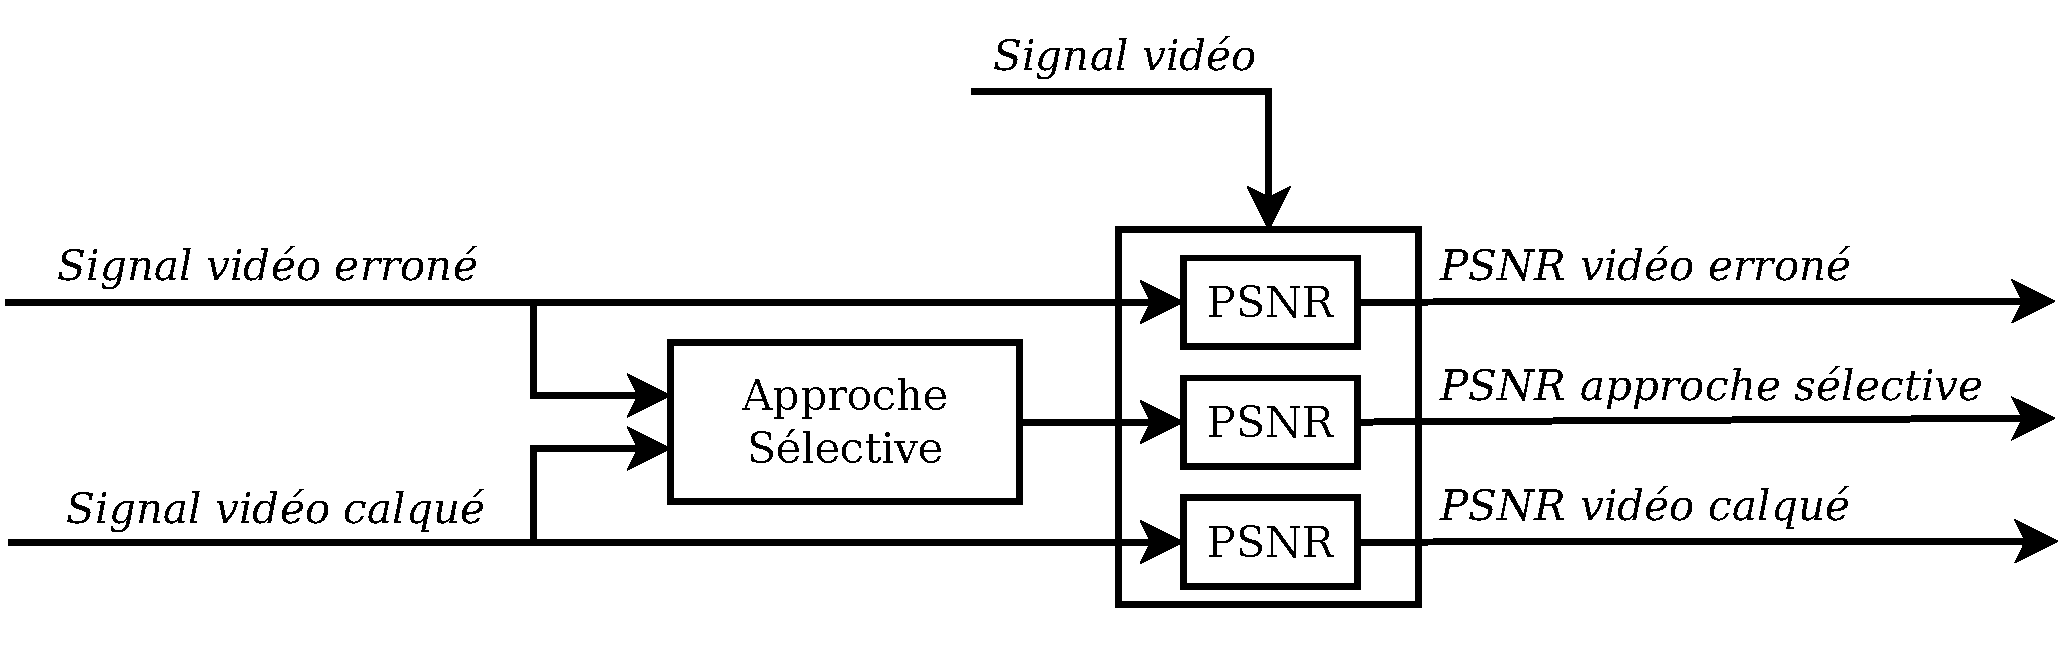
\includegraphics[width=0.75\linewidth]{images/SelectiveSetup.pdf}
}
\caption{Partie~2 de la Figure~\ref{fig-EncoderDecoder}. Configuration du banc
d'essai pour mesurer l'approche sélective basée SDMCB et MCB.}
\label{fig-SelectiveSetup}
\end{figure}
\DIFaddbegin \SC{Enlever la référence à la figure 1.2. le mentionner dans le texte toutefois. Aussi voir mes commentaires sur la figure 1.2 et les appliquer ici pour le nom décodeur partout ex PSNRerr, PSNRTC, etc. Aussi, trouver des noms aux valeurs de PSNR de chaque signal (faire une flèche qui sort des boites PSNR)}
\DIFaddend 

Tout d'abord, à l'aide du PSNR comme discriminant, nous mesurons la distribution\DIFaddbegin \SC{on calcule vraiment une distribution?}
\DIFaddend des meilleures dissimulations, entre le calque de la tranche et la tranche
corrompue. La \fig{fig-SelectiveSetup} démontre la configuration élaborée pour
obtenir ces mesures. On y \DIFdelbegin \DIFdel{comprend }\DIFdelend \DIFaddbegin \DIFadd{constate }\DIFaddend que le PSNR est mesuré par rapport au signal
vidéo de référence et qu'il est mesuré pour \DIFdelbegin \DIFdel{~: }\DIFdelend l'image résultante du décodage de
la tranche corrompue, le candidat de dissimulation basée sur le calque de la
tranche et le résultat des approches sélectives basées sur le SDMCB et MCB.

Les résultats mesurés \DIFaddbegin \DIFadd{sur le banc de tests proposé }\DIFaddend sont présentés à la \fig{fig-ScVsErroneous}. 
On y \DIFdelbegin \DIFdel{aperçoit qu'}\DIFdelend \DIFaddbegin \DIFadd{remarque }\DIFaddend une importante quantité de trames et \DIFaddbegin \DIFadd{de }\DIFaddend blocs erronés qui \DIFdelbegin \DIFdel{démontrent
}\DIFdelend \DIFaddbegin \DIFadd{possèdent
}\DIFaddend un PSNR supérieur aux calques de trames. \DIFdelbegin \DIFdel{Ce qui }\DIFdelend \DIFaddbegin \DIFadd{Cela }\DIFaddend s'explique par le fait \DIFdelbegin \DIFdel{, que}\DIFdelend \DIFaddbegin \DIFadd{que, dans ces cas, }\DIFaddend la
dégradation visuelle engendrée par la désynchronisation du décodeur est moins
importante que la variation temporelle par rapport à la trame précédente\DIFdelbegin \DIFdel{exploitée par }\DIFdelend \DIFaddbegin \DIFadd{; ce qui pénalise
 }\DIFaddend le calque de tranche. En lien avec les trois états d'un décodeur
\DIFdelbegin \DIFdel{décodant }\DIFdelend \DIFaddbegin \DIFadd{traitant }\DIFaddend une tranche corrompue, nous pouvons conclure que dans l'état~1, la
tranche endommagée va produire un meilleur résultat que le calquage de la
tranche. Dans l'état~2, la tranche endommagée va produire un résultat inférieur
à la tranche calquée. Finalement, à l'état~3, les deux sont équivalents. La
proportion de blocs compris dans les états~1 et 2, l'intensité de la dégradation
produite par le décodeur ainsi que la variation temporelle par rapport à la
trame précédente sont les facteurs qui déterminent laquelle des deux trames
\DIFdelbegin \DIFdel{sera }\DIFdelend \DIFaddbegin \DIFadd{constituera }\DIFaddend la meilleure dissimulation. \DIFaddbegin \SC{On veut vraiment dire la meilleure dissimulation ou plutôt la meileure alternative?}
\DIFaddend 

\begin{figure}[htb]
\fbox{\begin{varwidth}{\textwidth}\centering
\subfigure[Distribution des trames corrompues (ronds rouges) par rapport aux
trames calquées (ligne bleue)]{
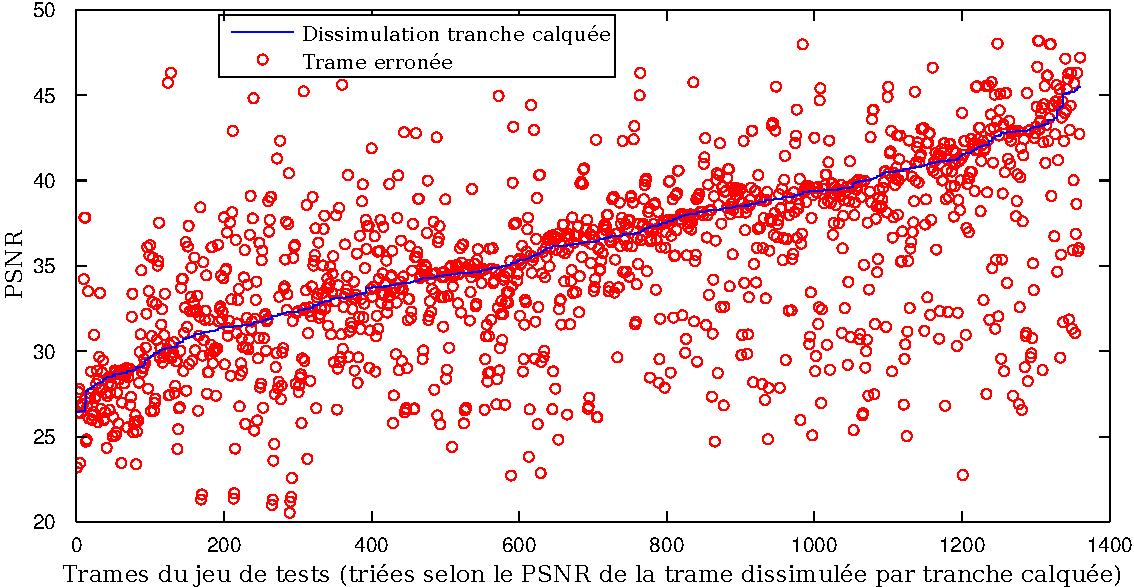
\includegraphics[width=0.97\linewidth]{images/scVsErroneous.pdf}
\label{fig-scVsErroneous}
}\\
\subfigure[Distribution des blocs issus des trames corrompues (ronds magenta)
par rapport aux blocs issus des trames calquées (ligne noire). À des fins de
visualisation, seulement un bloc sur dix est affiché.]{
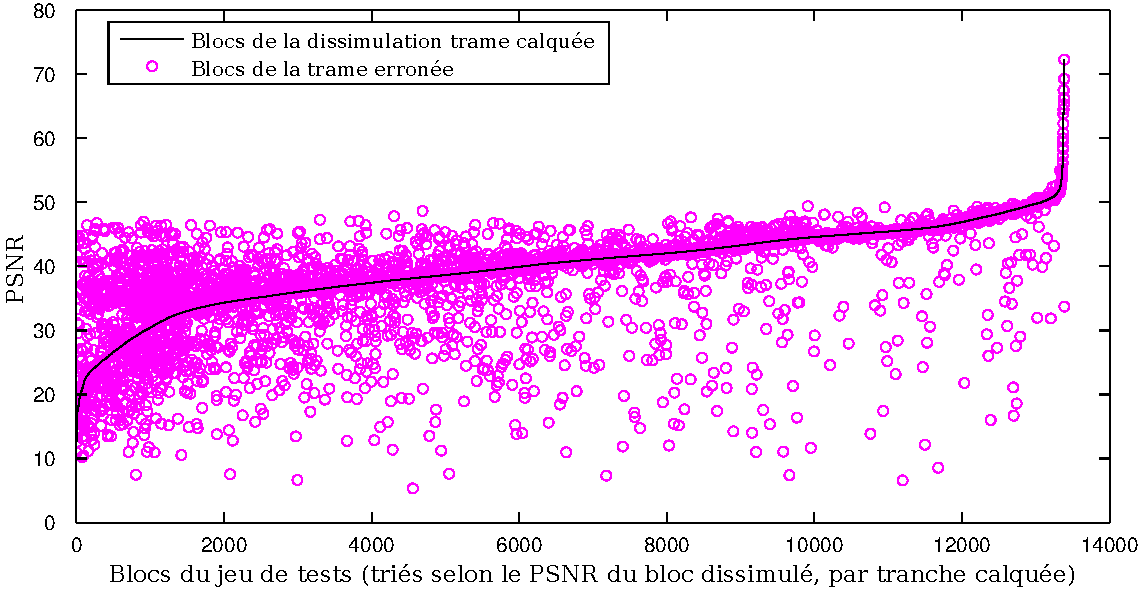
\includegraphics[width=0.97\linewidth]{images/ScVsErroneousBlocks.pdf}
\label{fig-scVsErroneousBlocks}
}
\end{varwidth}}
\caption{Visualisation de la distribution des valeurs du PSNR de la trame
erronée et de la dissimulation par tranche calquée.}
\label{fig-ScVsErroneous}
\end{figure}

Plus précisément, les mesures obtenues de notre banc d'essai nous permettent de
conclure que l'image résultante du décodage de la tranche corrompue offre un
PSNR plus élevé dans 44~\% des cas pour l'ordonnancement dispersé et 49~\% pour
l'entrelacé. Pour ces trames, on observe respectivement des gains moyens de
2.12~dB et 1.68~dB par rapport à leurs \DIFaddbegin \DIFadd{trames }\DIFaddend équivalentes \DIFdelbegin \DIFdel{calquer.  Tandis que }\DIFdelend \DIFaddbegin \DIFadd{calquées.  De manière similaire, }\DIFaddend les
blocs issus de trames corrompues sont supérieurs dans 42~\% des cas pour
l'ordonnancement dispersé et 49~\% pour l'entrelacé. Ces blocs produisent, pour
les approches d'ordonnancement précédentes, des gains moyens de 1.44~dB et
1.02~dB.\DIFaddbegin \SC{devrait-on avoir plus de graphiques en annexe comme montrer cela par débit ou taux d'arreur et voir la tendance?}
\DIFaddend 

Nous avons démontré, non seulement, qu'il est possible de réussir à décoder des
tranches erronées. Mais aussi qu'une quantité importante des images résultantes
exhibent une fidélité visuelle supérieure au calque de cette tranche (approche
couramment employée par le décodeur fourni avec le \ltCodec).

\begin{subsection}{Approche sélective SDMCB}
\label{sec-AnalyseSDMCB}
Maintenant, toujours avec la même configuration du banc de test, mesurons
l'aptitude du SDMCB à identifier le meilleur candidat entre la trame corrompue
et la dissimulation par tranche calquée. Pour ce faire, nous allons utiliser une
taille de bloc $B=16$ (vu notre indépendance au train de bits, nous ne
connaissons pas la taille exacte des blocs) et un seuil d'effet de bloc $T_b =
5000$.\DIFaddbegin \SC{Les gens vont te questionner sur l'origine du 5000. Il faut expliquer. pour la taille des blocs,  les MB 16x16 sont les plus souvent utilisés peu importe la norme. donner aussi la section dans laquelle la méthode SDMCB est présentée dans le mémoire. Quelques screenshot cas de trame calquée vs ton algo serait instructif}
\DIFaddend 

\begin{figure}[htb]
\fbox{\begin{varwidth}{\textwidth}\centering
\subfigure[Ordonnancement dispersé]{
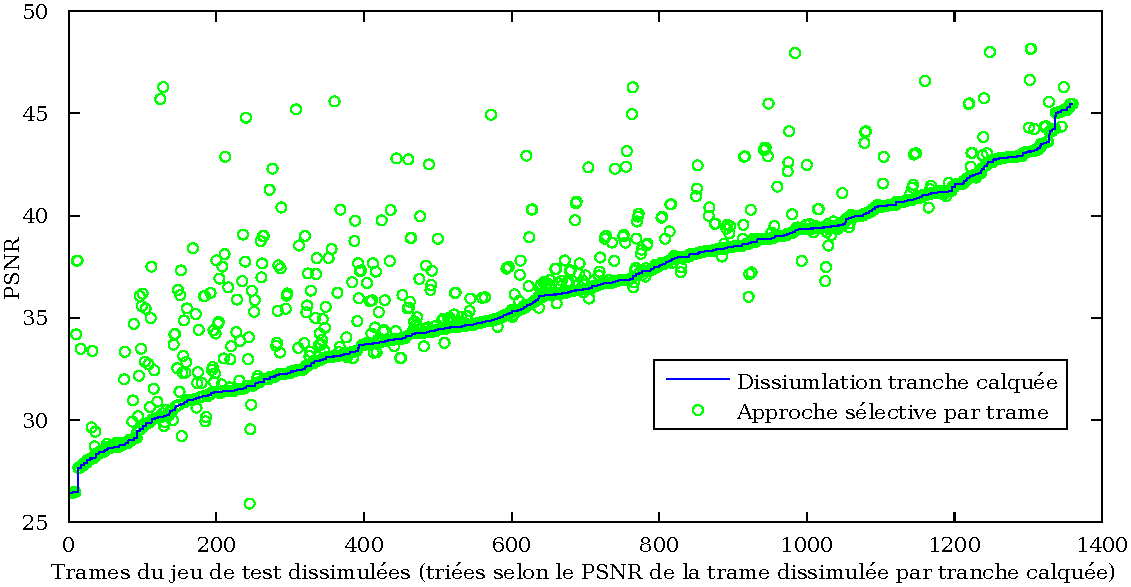
\includegraphics[width=0.97\linewidth]{images/selectiveSliceCopyDispersed.pdf}
\label{fig-sliceCopyDispersed}
}\\
\subfigure[Ordonnancement entrelacé]{
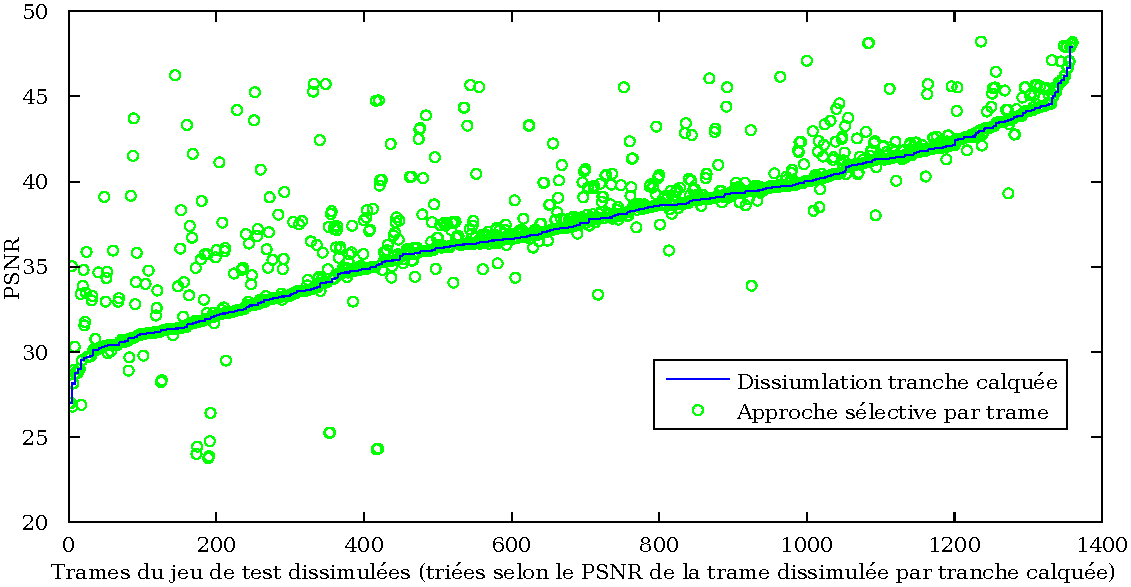
\includegraphics[width=0.97\linewidth]{images/selectiveSliceCopyInterleaved.pdf}
\label{fig-sliceCopyInterleaved}
}
\end{varwidth}} 
\caption{Visualisation de la distribution du PSNR de l'approche sélective basée
sur SDMCB (ronds verts) à l'égard de la dissimulation par tranche calquée (ligne
bleue).}
\label{fig-SelectiveSliceCopy}
\end{figure}\DIFaddbegin \SC{Ronds ou cercles?}
\DIFaddend 

Les résultats obtenus sont présentés à la \fig{fig-SelectiveSliceCopy}. La
\fig{fig-sliceCopyDispersed} témoigne que l'approche sélective, dans le cadre
d'un ordonnancement dispersé, fait le bon choix dans 81~\% des cas. Pour
ceux-ci, un gain moyen de 1.98~dB est mesuré, tandis que pour l'ensemble de la
séquence le gain moyen est de 0.72~dB. Les choix de l'approche sélective offrent
un PSNR supérieur aux trames dissimulées par calquage de tranche dans 31~\% des
cas. Pour la \fig{fig-sliceCopyInterleaved}, la bonne trame est choisie dans
86~\% des cas, résultant dans un gain moyen de 1.24~dB pour celles-ci. Sur
l'ensemble des trames, le gain moyen est de 0.65~dB et un PSNR supérieur au
calquage de trame est obtenu dans 43~\% des cas.

\end{subsection}
\begin{subsection}{Approche sélective MCB}
\label{sec-AnalyseMCB}
Le niveau de granularité plus fin de l’approche sélective MCB est son attrait
principal. En remplaçant uniquement les blocs endommagés, on maximise l’usage
des données correctement décodées.

Sans altérer la configuration de notre banc de test, nous mesurons l'aptitude du
MCB à identifier le meilleur bloc candidat entre ceux provenant de la trame
corrompue et ceux de la dissimulation par tranche calquée. Pour ce faire, nous
allons utiliser une taille de bloc $B=16$ et un seuil d'effet de bloc $T_b =
5000$.

\begin{figure}[htb]
\fbox{\begin{varwidth}{\textwidth}\centering
\subfigure[Ordonnancement dispersé]{
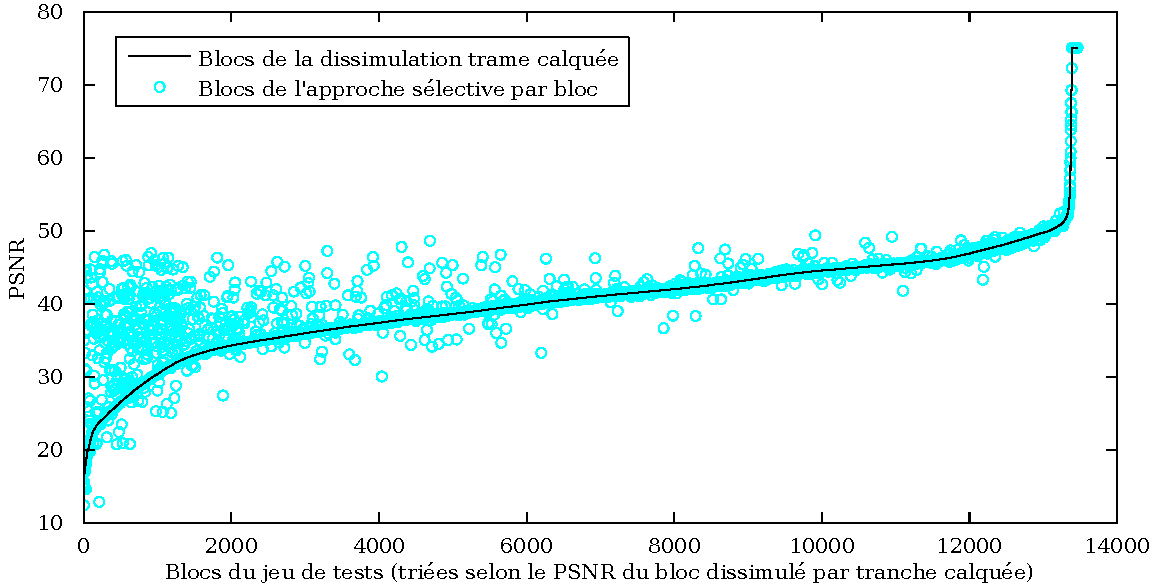
\includegraphics[width=0.97\linewidth]{images/SelectiveSliceCopyBlocksDispersed.pdf}
\label{fig-selectiveSliceCopyBlockDispersed}
}\\
\subfigure[Ordonnancement entrelacé]{
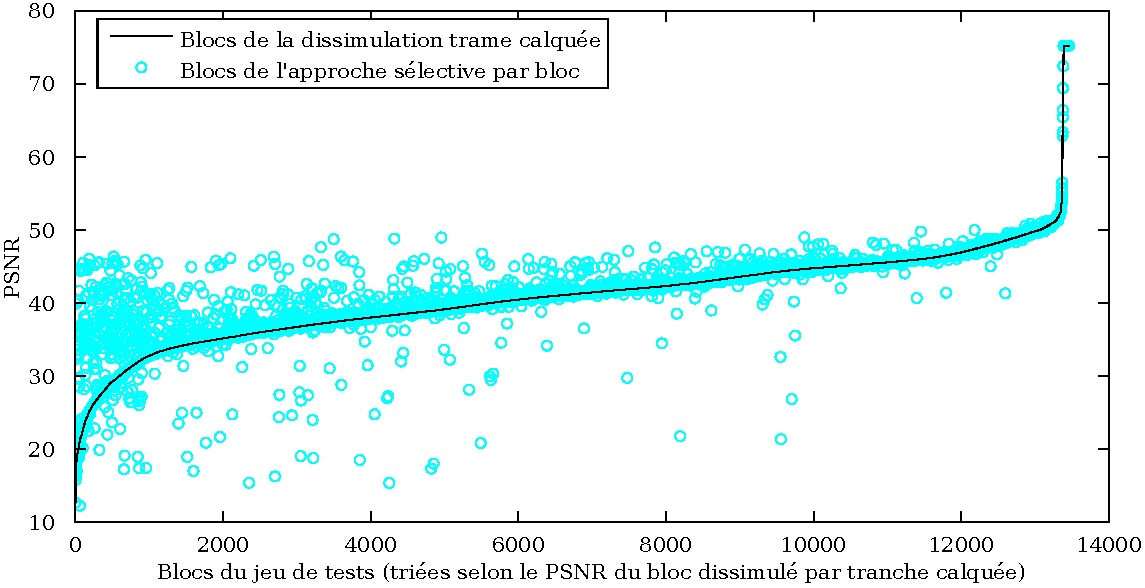
\includegraphics[width=0.97\linewidth]{images/SelectiveSliceCopyBlocksInterleaved.pdf}
\label{fig-selectiveSliceCopyBlockInterleaved}
}
\end{varwidth}}
\caption{Visualisation de la distribution du PSNR issue des blocs résultants de
l'approche sélective basée sur MCB (ronds verts) à l'égard de ceux produits par
la dissimulation par tranche calquée (ligne bleue).}
\label{fig-SelectiveSliceCopyBlocks}
\end{figure}
\DIFaddbegin \SC{vert ou turquoise/cyan?}
\DIFaddend 

Les résultats obtenus sont présentés à la \fig{fig-SelectiveSliceCopyBlocks}.
La \fig{fig-selectiveSliceCopyBlockDispersed} démontre que l'approche sélective
MCB choisit le bon bloc dans 88~\% de cas. Ce qui produit un gain moyen de
0.86~dB sur l'ensemble des trames avec un ordonnancement de type dispersé.
Pour l'ordonnancement entrelacé (\fig{fig-selectiveSliceCopyBlockInterleaved}),
l'approche sélective MCB effectue le bon choix dans 91~\% des cas, permettant un
gain moyen de 0.69~dB. \DIFaddbegin \SC{pourquoi pas toutes les stats comme SDMCB somme le 1.98 dB et 1.24dB? Est-ce par ce que tu ne sais plus à quel trame appartient chaque bloc?}
\DIFaddend \end{subsection}

À l'aide de la \fig{fig-FrameDistribution}, nous sommes en mesure d'analyser
la distribution des PSNR résultants~: de la trame erronée, de la dissimulation
par tranche calquée et des approches sélectives. Cette figure expose la
variation du nombre de trames selon des intervalles de 5~dB de PSNR. Ces
intervalles s'étalent de 20~dB à 50~dB, permettant ainsi de visualiser la
variation de la qualité visuelle issue de chaque approche. Commençons l'analyse
en soulignant la présence d'une importante quantité de trames erronées dans les
intervalles de faible qualité, où le PSNR est inférieur à 30 (les intervalles
centrés autour de 20 et 25). Pour ces intervalles, nous constatons, autant dans
l'histogramme de la \fig{fig-SelectiveHistDispersed} que
\ref{fig-SelectiveHistInterleaved}, que la majorité de ces trames sont
dissimulées par le calquage de tranche et les approches sélectives. Poursuivons
l'analyse des approches sélectives avec le constat suivant, pour l'intervalle
centré autour de 30~dB, le nombre de trames liées aux approches sélectives est
inférieur à celui lié à la dissimulation par tranche calquée. Cette observation
n'est pas due à une perte de qualité, mais bien à une augmentation de la
qualité, car on retrouve ces trames dans les intervalles supérieurs. Pour ces
intervalles, les approches sélectives produisent un plus grand nombre de trames
que la dissimulation par tranche calquée. Grâce à ces observations, nous sommes
en mesure de conclure que les approches sélectives produisent de meilleurs
résultats en exploitant les trames erronées de haute qualité visuelle, tout
en évitant les trames erronées de mauvaise qualité. En ce qui a trait à la
comparaison des approches sélectives, l'approche sélective MCB offre un plus
grand nombre de trames de qualité visuelle pour les intervalles de 35~dB et
40~dB vis-à-vis SDMCB. Cependant, cette dernière se reprend dans l'intervalle
de 45~dB. Cette reprise est attribuée au fait que le remplacement de blocs
sporadique dans une trame peut engendrer une perte de qualité causée par le
mauvais arrimage des valeurs de pixels en frontière de bloc. Cette légère
dégradation réduit le nombre de trames de très haute qualité. \DIFaddbegin \DIFadd{Toutefois à des niveaux de 40dB et plus, la différence de qualité est souvent imperceptible. }\SC{Expliquer que le PSNR est saturé à une certaine valeur et dire laquelle}
\DIFaddend 

\begin{figure}[htb]
\fbox{\begin{varwidth}{\textwidth}\centering
\subfigure[Ordonnancement dispersé]{
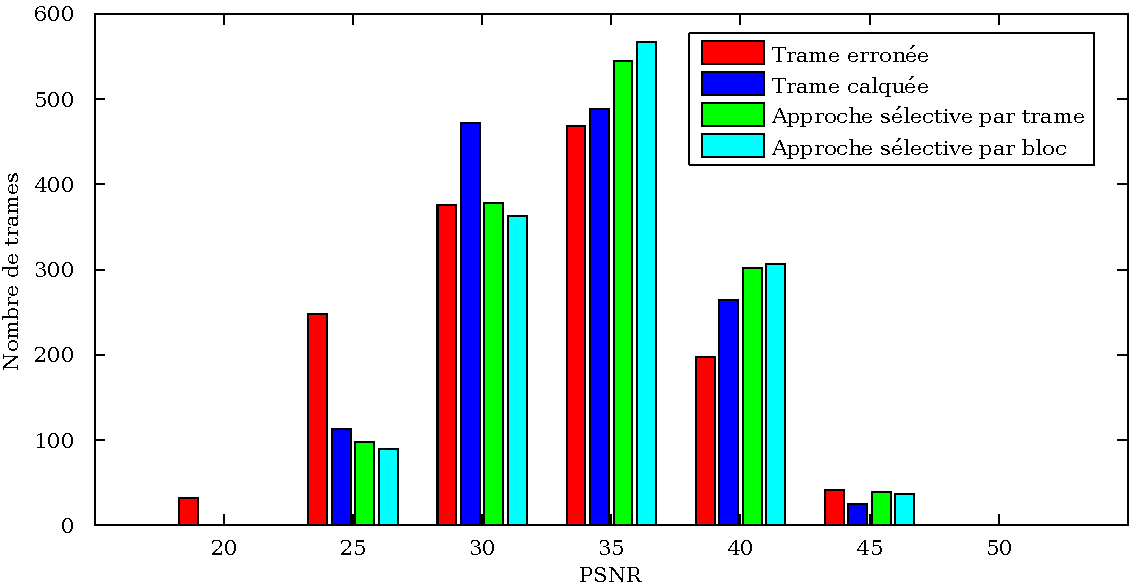
\includegraphics[width=0.97\linewidth]{images/SelectiveHistDispersed.pdf}
\label{fig-SelectiveHistDispersed}
}\\
\subfigure[Ordonnancement entrelacé]{
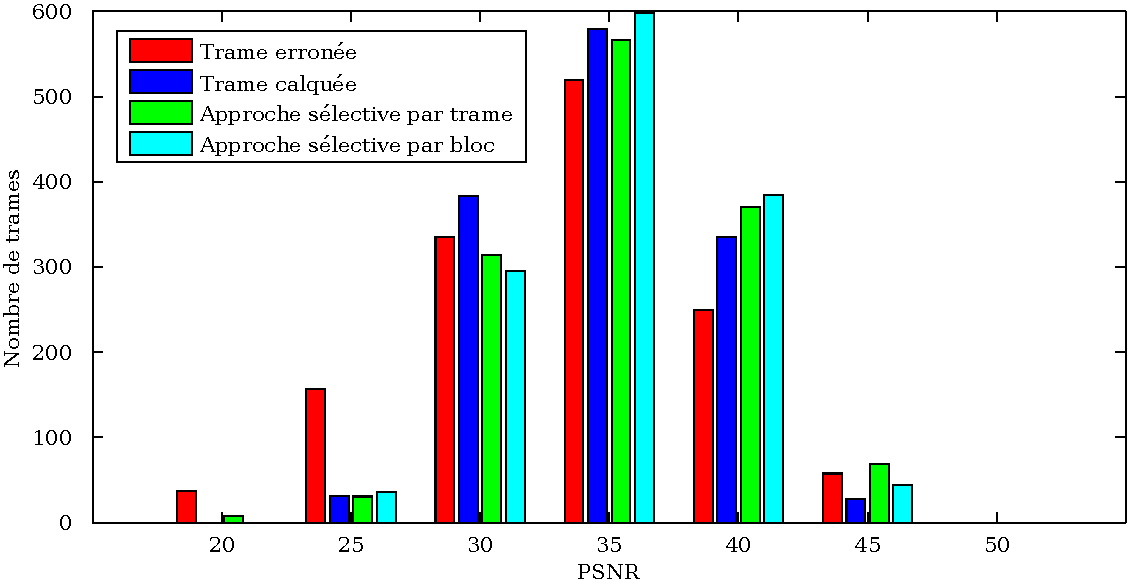
\includegraphics[width=0.97\linewidth]{images/SelectiveHistInterleaved.pdf}
\label{fig-SelectiveHistInterleaved}
}
\end{varwidth}}
\caption{Histogrammes des PSNR des trames, avec des intervalles de 5~dB, centrés
à chaque incrément de 5~dB, à partir de 20~dB. Les trames considérées sont
celles résultantes~: du décodage de la trame erronée (rouge), du calquage de
tranche (bleu), de l'approche sélective par tranche (vert) ainsi que
l'approche sélective par bloc (cyan).} 
\label{fig-FrameDistribution}
\end{figure}

\begin{table}[!htb]
\caption{Résumé du PSNR moyen obtenu par les diverses approches présentées dans
cette section \DIFaddbeginFL \DIFaddFL{sur le jeu de tests}\DIFaddendFL .}
\label{tab-ResumeSelectif}
\small
\centering
\begin{tabular}{| l | c | c |}
 \hline
 \textbf{Approche} & \textbf{PSNR Moyen}& \textbf{PSNR Moyen}\\
 &\textbf{dispersé (dB)}&\textbf{entrelacé (dB)}\\
 \hline
 Encodée (sans erreur) & 41.218222 & 41.200377\\
  \hline
 Sélective par bloc (avec référence) & 37.689039 & 38.528986\\
  \hline
 Sélective par tranche (avec référence) & 37.117712 & 38.082769\\
  \hline
 Sélective MCB & \textbf{37.034840} & \textbf{37.951004}\\
  \hline
 Sélective SDMCB & \textbf{36.901414} & \textbf{37.911514}\\
  \hline
 Dissimulation tranche calquée & 36.179630 & 37.263033\\
  \hline
 Trame corrompue & 35.068784 & 36.075526\\
 \hline   
\end{tabular}
\end{table}

\DIFaddbegin \SC{Il faut présenter et analyser le tableau 1.1. Il manque aussi une petite conclusion au chapitre}

\DIFaddend \end{section}

\bibliographystyle{bibETS}
\bibliography{resultats}

\end{chapter}

\end{document}